\section{Leader Election} % (fold)
\label{sec:leader_election}
In this section we will start describing the component of leader election done in Raft. Then describe and discuss the challenges when implementing this.

\subsection{Leader election in Raft}
As mentioned in section \ref{sec:raft} one of the two main components of Raft is its leader election. After a successful leader election the given leader is responsible of replicating commands it receives from a client to the rest of the followers called log replication, which is explained in section \ref{sec:log_replication}. All servers contain an implementation of Raft, having a log of commands requested by clients. A server can be in three states: leader, candidate or follower. Most of the servers in the system will be in the 'follower' state in which they act as an active part receiving heart beat messages from the current leader. At most one leader exists at any given moment denoted 'a term'. The term is incremented each time a new leader is elected. In distributed systems the term is the systems logical clock in which any entry in the servers logs has a term attached to it in order to know when that value has been replicated to it.

Figure~\ref{fig:election_example} illustrates the scenario in which a leader is elected:

In the beginning of the illustration, on initial system startup, every server is a follower until $P1$ times out, because it has not received any valid heart beat messages from a leader, and becomes a candidate. If this candidate receives a majority of votes it transitions to the leader state after which it has the responsibilities of a leader as described in section \ref{sec:raft}. The leader claims its leadership by sending out heartbeats, where if a server receives a heartbeat request from another server it is instantly converted to follower and recognizes the source as leader.

\begin{figure}[ht!]
\centering
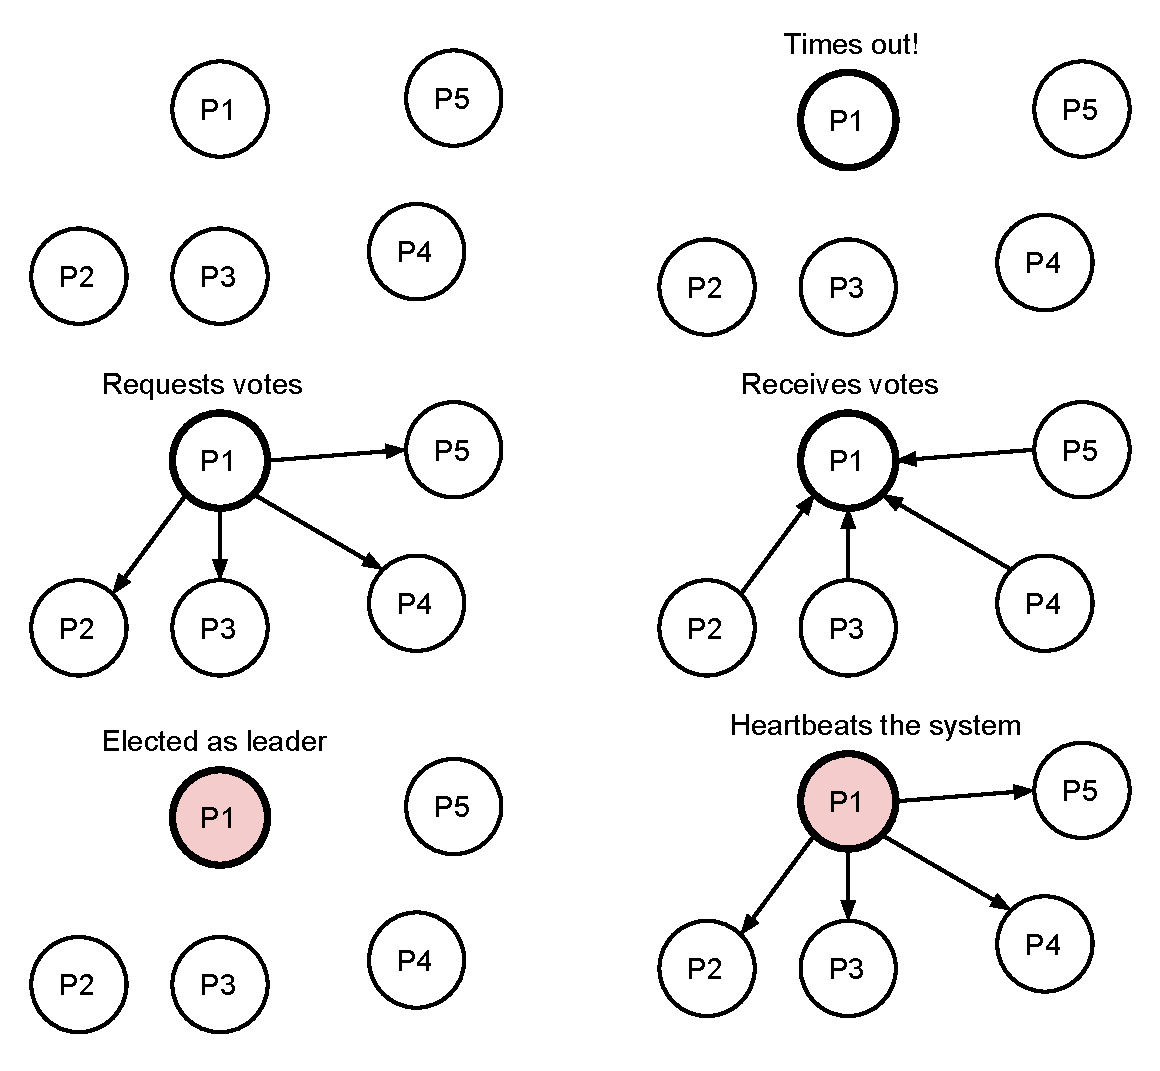
\includegraphics[scale = 0.5]{election-example.pdf}
\caption{A simple scenario where 5 servers are to obtain consensus by first electing a leader.}
\label{fig:election_example}
\end{figure}

Figure~\ref{fig:failure_example} shows how Raft will tolerate a faulty leader. Here we see that the leader $P1$ fails by crashing. $P4$ then times outs and initiates a new election.

\begin{figure}[ht!]
\centering
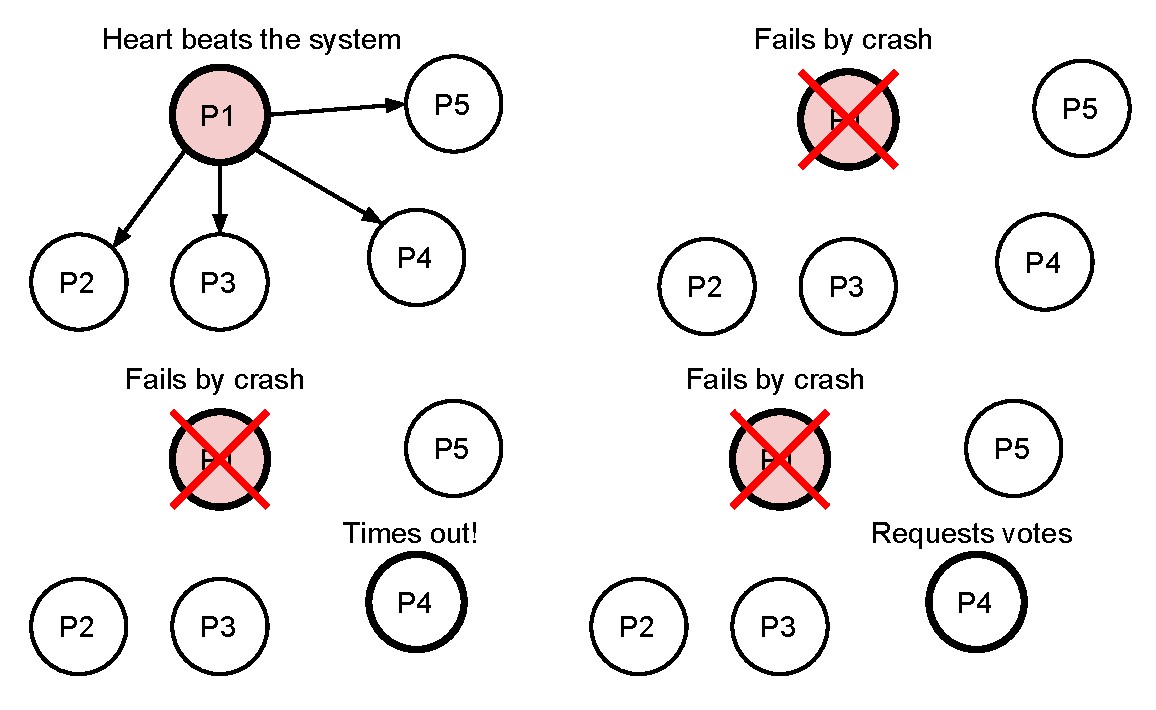
\includegraphics[scale = 0.5]{failure-example.pdf}
\caption{A simple scenario where a leader $P1$ crashes after which $P4$ times out and start a new election.}
\label{fig:failure_example}
\end{figure}

It should also be noted that upon transitioning to the candidate state and requesting votes, another server might have been requesting votes before this. In this situation the candidate would receive a heart beat message from a leader with a term at least as large as its own, after which is transitions back to follower.
The situation in which a majority vote is not achieved by any candidate, the candidates will issue yet another election once they time out again. And in order to avoid split these kinds of situation too frequently i.e. split votes, Raft gives each server an arbitrary time out within a given interval.

It should also be noted that since the availability, provided by Raft, relies on the majority votes and only non-Byzantine failures, the algorithm can thus only uphold these properties in a network where $3F \leq N$, where $F$ is the amount of failures and $N$ is the amount of processes in the system.~\cite{Fischer}

Looking back at the Two Generals Problem, Raft is only be able to solve the problem if a majority vote would be possible, which it is not. So in order to solve this problem when utilising Raft, one must add another general to the scenario such that there are an uneven number of generals in the system. We should also modify the problem such that the messenger always tells the truth (i.e. cannot suffer from Byzantine failures). Now that we have three generals and an ``uncapturable'' messenger, they will reach consensus by finding a leader after which he decides when to launch the attack.

% TODO: explain figure of different states (maybe take it from the Raft Paper)

% subsection leader_election_in_raft (end)

\subsection{Implementation} % (fold)
\label{sub:leader_election_implementation}

Our Raft implementation consists of two major parts:

\begin{enumerate}
  \item An election timer that is resetted with a random time in a specificed interval
  \item RequestVote RPC implementation that with methods for handling invokation and receiving RequestVote RPC request and response
\end{enumerate}

\subsubsection{Election Timer} % (fold)
\label{ssub:election_timer}

The election timer is implemented by keeping state of the amount of milliseconds left and decrement this value every millisecond using the JavaScript function \verb$setInterval$. The timer is then reset in five situations:

\begin{itemize}
  \item On initialization
  \item On restart
  \item When receiving an AppendEntries RPC
  \item When it has started an election
  \item When it has voted for another candidate
\end{itemize}

% subsubsection election_timer (end)

\subsection{RequestVote RPC} % (fold)
\label{sub:requestvote_rpc}

If the election timer reaches zero it will start an election by sending a Remote Producure Call (RPC) request called \emph{RequestVote RPC}, where each server responds whether or not it will grant a vote to the candidate. As the votes are independent to each server they can be send out in parallel as specified in the Raft paper. Since our implementation is a simulation with objects instead of processes or servers and JavaScript does not have threads, it is not possible to do true parallel computing. But since it is an simulation we simluate parallel requests with the JavaSript method \verb$setTimeout$, which delays the execution of a given function. To make the simulation more like real requests, they are delayed given by a random amount of milliseconds in a given interval.

This implementation is fine for the implementation, but since we also wants to verify the implementation through tests, it is not convenient to make the election random since you cannot assert a random election result. It would be possible to assert a given property such as ``assertion that there is at most one leader after x seconds''. Although this could be a viable test it is not convient either since it will make the tests slow and thereby slow down the development flow.

In order to easily test the execution of the RequestVoteRPC, we have made a protocol for communicating between servers in Raft. The protocol is an object that delegates a method call to a target and is injectable in the Server object. The delayed implementation explained above is seen in the protocol object \verb$DirectAsync$. The protocol used in testing will call methods directly on the target object and is called \verb$Direct$.

% subsection requestvote_rpc (end)

% - Problems
%   - Intro:
%     - Random election timer
%     - Parallel RPC's (RequestVote)
%     -
%   - Raft uses a randomly initiated timeout to do election:
%     - Every follower has an election timer given by a random time interval that
%       is reset with a new random time given by a random interval between t_1 and t_2.
%   - Problem:
%     - Hard to test, because:
%       a. you cannot assert a random result.
%       b. you do not want tests to be dependent on a time interval, because then you have slow tests
%       c. you cannot guarantee any test will pass every time if it is random (every test run is different)
%   -
%
% subsection implementation (end)

% section leader_election (end)
